\documentclass[a4paper, 10pt]{article}
\usepackage[ascii]{inputenc}
\usepackage[T1]{fontenc}
\usepackage[romanian,english,ngerman]{babel}
\usepackage{amsmath}
\usepackage{amssymb,amsfonts,textcomp}
\usepackage{color}
\usepackage{array}
\usepackage{hhline}
\usepackage{hyperref}
\hypersetup{pdftex, colorlinks=true, linkcolor=blue, citecolor=blue, filecolor=blue, urlcolor=blue, pdftitle=, pdfauthor=, pdfsubject=, pdfkeywords=}
\usepackage[pdftex]{graphicx}

%%%% Cosmin

\usepackage[a4paper, margin=2.5cm]{geometry}
\renewcommand*{\familydefault}{\sfdefault} %Sans Serif font
\renewcommand{\sfdefault}{phv} % Arial
\setlength{\parindent}{0pt} % no indentation for paragraphs
\setlength{\tabcolsep}{70pt} % table inter-column spacing

%%%%

% List styles
\newcommand\liststyleLv{%
\renewcommand\theenumi{\arabic{enumi}}
\renewcommand\theenumii{\arabic{enumii}}
\renewcommand\theenumiii{\arabic{enumiii}}
\renewcommand\theenumiv{\arabic{enumiv}}
\renewcommand\labelenumi{\theenumi.}
\renewcommand\labelenumii{\theenumii.}
\renewcommand\labelenumiii{\theenumiii.}
\renewcommand\labelenumiv{\theenumiv.}
}
\newcommand\liststyleLSi{%
\renewcommand\theenumi{\arabic{enumi}}
\renewcommand\theenumii{\arabic{enumii}}
\renewcommand\theenumiii{\arabic{enumiii}}
\renewcommand\theenumiv{\arabic{enumiv}}
\renewcommand\labelenumi{\theenumi.}
\renewcommand\labelenumii{\theenumii.}
\renewcommand\labelenumiii{\theenumiii.}
\renewcommand\labelenumiv{\theenumiv.}
}

% Footnote rule
\setlength{\skip\footins}{0.047in}
\renewcommand\footnoterule{\vspace*{-0.0071in}\setlength\leftskip{0pt}\setlength\rightskip{0pt plus 1fil}\noindent\textcolor{black}{\rule{0.25\columnwidth}{0.0071in}}\vspace*{0.0398in}}

% Pages styles
\makeatletter
\newcommand\ps@Standard{
  \renewcommand\@oddhead{}
  \renewcommand\@evenhead{}
  \renewcommand\@oddfoot{}
  \renewcommand\@evenfoot{}
  \renewcommand\thepage{\arabic{page}}
}

\makeatother
\pagestyle{plain}
\title{}
\author{}
\date{2013-04-08}

\begin{document}
{\raggedleft\bfseries
MACHETA 3
\par}

{\bfseries
Contractor: \foreignlanguage{romanian}{Universitatea din Bucure\c{s}ti}}

{\textbf{Cod fiscal: 45055002}

\bigskip

\bigskip

{\bfseries

\begin{tabular}{@{}l l}
Avizat,&De acord,\\
Comisia de monitorizare&DIRECTOR PLAN SECTORIAL\\
\end{tabular}
}

\bigskip

Ordonator de credite, Secretar de Stat

Prof.univ.dr. Tudor Prisecaru

\bigskip

\bigskip

\bigskip

MEMBRII

\medskip

\medskip

MONITOR PROIECT

Daniela Dinic\u{a}

\bigskip

\bigskip

\bigskip

\bigskip

{\centering\bfseries
RAPORT DE ACTIVITATE AL FAZEI
\par}

\bigskip

\bigskip

{\bfseries
Contractul nr.: 5S / 27.07.2012}

{
\textbf{Proiectul: }
\textit{`` Sistem informatic integrat pentru identificarea, arhivarea \c{s}i diseminarea bazelor de date \c{s}i a indicatorilor din
cercet\u{a}rile sociale ''}}

%TODO Numarul fazei !
%TODO Titlul fazei !
{
\textbf{Faza: }
Nr. III cu titlul
\textit{`` Dezvoltarea software, pachet 2: biblioteci nucleu, sistem template, autentificare. Raport privind modernizarea dot\u{a}rilor ''}}

{\textbf{Termen:} 15.08.2013}

\medskip

\section{Obiectivul proiectului}

{
\foreignlanguage{english}{Realizarea }\foreignlanguage{romanian}{unei arhive electronice integrate care s\u{a}
con\c{t}in\u{a} \c{s}i s\u{a} distribuie c\^at mai multe dintre datele sociologice acumulate \^in Rom\^ania.}}

\medskip

Sistemul trebuie s\u{a} ofere cercet\u{a}torilor \^in domeniul \c{s}tiin\c{t}elor sociale instrumentele necesare pentru
trecerea \^in revist\u{a}, compararea, sintetizarea, ad\u{a}ugarea datelor sociologice de interes. Operatorii interni
ai arhivei vor c\u{a}uta, identifica \c{s}i acumula date sociologice disponibile \^in Rom\^ania.

\medskip

Arhiva va fi integrat\u{a} \^in Consiliul European al Arhivelor de Date Sociale (CESSDA) asigur\^andu-se un schimb
continuu bidirec\c{t}ional de informa\c{t}ie.

\section{Rezultate preconizate pentru atingerea obiectivului}

\begin{enumerate}
\item {
Sistem informatic de arhivare (stocare, catalogare plus proceduri \c{s}i capacit\u{a}\c{t}i de identificare \c{s}i
accesare) \foreignlanguage{romanian}{\c{s}}i diseminare a datelor sociale produse de pia\c{t}a cercet\u{a}rii sociale
din Rom\^ania.}
\item {
Asigurarea procedurilor de securizare a accesului la datele arhivate, ca urmare a investi\c{t}iilor \^in hardware
\foreignlanguage{romanian}{\c{s}}i software pe parcursul proiectului;}
\item {
\foreignlanguage{romanian}{Arhiva }va func\c{t}iona inclusiv ca o banc\u{a} de date sociale, dat fiind faptul c\u{a}
produc\u{a}torii de date nu au nici capacit\u{a}\c{t}ile tehnice nici \foreignlanguage{romanian}{cunoa\c{s}terea}
necesar\u{a} depozit\u{a}rii, catalog\u{a}rii \c{s}i acces\u{a}rii cercet\u{a}rilor realizate, pe termen lung;}
\item {
Facilitarea accesului comunit\u{a}\c{t}ii de cercetare din Rom\^ania la datele produse \^in ultimii 20 de ani pe
pia\c{t}a na\c{t}ional\u{a} de profil, dar \c{s}i la cele europene, ca urmare a conect\u{a}rii arhivei la CESSDA-ERIC
(arhiva fiind deja membru al CESSDA);}
\item {
Facilitarea accesului comunit\u{a}\c{t}ii de cercetare interna\c{t}ionale la datele produse \^in Rom\^ania prin
intermediul CESSDA va aduce de asemenea mari beneficii interna\c{t}ionaliz\u{a}rii cercet\u{a}rii sociale din
Rom\^ania;}
\item {
Articole de specialitate/comunic\u{a}ri \c{s}tiin\c{t}ifice menite a face cunoscute pe plan na\c{t}ional \c{s}i
interna\c{t}ional beneficiile sistemului implementat ca urmare a derul\u{a}rii sale.}
\end{enumerate}

\section{Obiectivul fazei}

%TODO Obiectivul fazei, cf. documentatiei proiectului 

Implementarea unor componente necesare pentru interfata publica.

\section{Rezultate preconizate pentru atingerea obiectivului fazei}

%TODO Rezultate ale fazei, cf. documentatiei proiectului

Completarea bibliotecilor nucleului aplicatiei, initializarea sistemului de
template, implementarea modulului de autentificare a utilizatorilor interfetei
web, debutul modulului de navigare prin arhiva de date.

\section{Rezumatul fazei}

\medskip

\subsection*{Biblioteci nucleu}

\medskip

Aplicatia RODA respecta principiile unei aplicatii web moderne, de tip MVC. Suplimentar, pe langa cele 3 niveluri specifice unei astfel de aplicatii, RODA are definit un nivel de servicii, care permite izolarea modelului fata de controllere si specificarea de drepturi de acces personalizate (prin liste de control al accesului - ACL). Exista servicii disponibile expuse aplicatiei ca JavaBeans, precum cele pentru: 
indexare si cautare, file-repository, integrarea unui motor statistic, executia asincrona sau programata de task-uri etc. 
Au fost definite controllere corespunzand unui sablon de interfata de tip \emph{CRUD}
(Create / Read / Update / Delete), pentru fiecare clasa din model. 
In controllere se fac apeluri catre nivelul de servicii. 
Au mai fost definite si controllere pentru a servi continut de baza in format JSON.

\medskip

Componentele dezvoltate in cadrul etapelor anterioare ale proiectului au fost completate cu functionalitati suplimentare, printre scopurile carora amintim furnizarea anumitor servicii si asigurarea suportului pentru activitatile viitoare. In acest sens, in clasele domeniului au fost implementate metode dintre care mentionam: verificarea egalitatii dintre instante, generarea unor valori hash corespunzatoare datelor stocate in cadrul instantelor si testarea existentei unor entitati in baza de date. Pe langa utilitatea lor in cadrul etapei curente, aceste metode vor servi ulterior componentei care va realiza importul de studii in baza de date si vor asigura unicitatea datelor in raport cu modelul conceptual. 

\medskip

Dintre elementele adaugate in cadrul nucleului aplicatiei se disting controller-erele si serviciile care asigura legatura dintre interfata aplicatiei si baza de date. Astfel, au fost implementate metode de recuperare a datelor corespunzatoare claselor domeniului, conform unor cerinte specifice, sub forma unor fisiere de tip JSON care servesc vizualizarii prin intermediul interfetei, intr-un mod care usureaza intelegerea lor de catre utilizator. Din categoria acestor servicii au fost implementate cele care sunt necesare functionarii componentei DataBrowser a interfetei. Ulterior, aceste servicii vor fi extinse cu cele prevazute in cadrul celorlalte componente ale aplicatiei. Pe langa partea de controller-e ce asigura legatura dintre nivelurile arhitecturale ale aplicatiei, bibliotecile nucleu vor fi extinse cu clase care vor gestiona relatia cu motorul statistic R si cu platforma de cautare Solr.

\medskip

\subsection*{Sistemul de template-uri}

\medskip

Se utilizeaza o combinatie intre framework-ul de template-uri Apache Tiles si pagini JSPX.

\medskip

Apache Tiles (\url{http://tiles.apache.org/}) este un framework software pentru templating construit pentru a simplifica dezvoltarea de aplicatii interfete web.
Tiles permite dezvoltatorilor sa defineasca fragmente de pagini care pot fi asamblate intr-o pagina intreaga in timpul rularii. 
Aceste fragmente, sau 'pl\u{a}cu\c{t}e', pot fi folosite la fel de simplu ca incluziuni/importuri (in scopul de a reduce redundanta elementelor comune de pagina) sau incorporate in alte pl\u{a}cu\c{t}e pentru a dezvolta o serie de \c{s}abloane reutilizabile. 
Aceste template-uri simplific\u{a} realizarea unor aspecte vizuale \c{s}i de interac\c{t}iune consistente pentru intreaga aplicatie web.

\medskip

Fisierele JSPX din aplicatie reprezinta pagini JSP sau snippet-uri JSP (reprezentand fragmente de pagina) ce sunt XML-uri valide si utilizeaza suplimentar mai multe librarii de tag-uri specifice Spring si Spring Roo (de ex. pt. meniu si itemii sai, form-uri si actiuni asociate uzuale, campuri din form-uri, multi-language, themes, paginare)
precum si framework-ul Dojo Toolkit (\url{http://dojotoolkit.org/}) pentru componente ale interfetei web (tabele, grid-uri si alte componente in pagina).

\medskip

Sistemul de template-uri dezvoltat permite:
\begin{itemize}
\item {\textbf{internationalizare}} - realizarea interfetei in mai multe limbi (cel putin rom\^{a}n\u{a} si englez\u{a}, intre care se poate alterna)
\item {\textbf{themes}} - aspecte vizuale diferite (de ex. pt. rezolutii diferite ale dispozitivelor de vizualizare, pt. utilizatori cu deficiente vizuale etc.)
\end{itemize}

A fost realizata si o componenta de interfata care permite upload-ul de fisiere, aceasta bazandu-se pe un serviciu dezvoltat in aplicatia server (cf. API-ului FileStore definit in faza 2 a proiectului).

\medskip

\subsection*{DataBrowser}

\medskip

DataBrowser este componentul central al interfetei publice RODA. Prin intermediul acestuia, utilizatorii vor
interactiona cu baza de date de studii, vor cauta datele care ii intereseaza si vor putea accesa datele identificate,
in functie de drepturile pe care le au.

\medskip

DataBrowser-ul va evolua pe toata durata dezvoltarii sistemului RODA, odata cu adaugarea noilor caracteristici pe care
le presupune procesul de dezvoltare. In aceasta faza, componentul permite ordonarea studiilor dupa ani sau cataloage si
vizualizarea datelor fiecarui studiu in parte.

\medskip

DataBrowser-ul este compus din doua regiuni, o regiune de cautare/sortare a seturilor de date si o regiune de
vizualizare a detaliilor elementelor selectate in panoul din dreapta.

\medskip

\begin{figure}[h!tb]
\centering
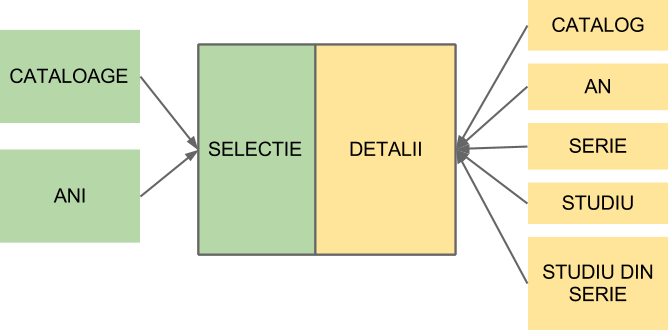
\includegraphics[width=\textwidth]{roda_databrowser-img001.png} 
\end{figure}

\medskip

Cele doua regiuni sunt construite ca doua containere care comunica intre ele. Fiecare dintre containere poate contine
mai multe tipuri de ecrane. In stadiul actual al dezvoltarii, studiile pot fi ordonate dupa ani sau dupa catalogul din
care fac parte, astfel incat, ecranele din containerul de ordonare corespund acestor doua variante. In containerul din
partea dreapta, in functie de selectia utilizatorului, se pot incarca urmatoarele ecrane:

\begin{itemize}
\item
{\textbf{catalog}}
- ecranul care prezinta informatii despre catalog (numele catalogului, descrierea acestuia precum si lista
studiilor care fac parte din catalogul curent)
\item
{\textbf{an}}
- ecranul care prezinta informatii despre anul selectat (studiile care au fost incepute in acest an)
\item
{\textbf{serie}}
- ecranul care prezinta informatii despre seria selectata (metadatele acesteia precum si studiile care fac parte
din seria respectiva)
\item 
{\textbf{studiu}}
- ecranul care prezinta informatii despre studiul selectat (metadate, variabile plus alte informatii atasate, in
functie de continutul bazei de date si drepturile utilizatorului curent).
\item
{\textbf{studiu din serie}}
- ecran special pentru un studiu care face parte dintr-o serie. Acest ecran este o combinatie intre
ecranul pentru un studiu si ecranul pentru o serie, in principal prezinta metadatele si datele studiului curent, dar,
afiseaza la cerere si metadatele seriei din care acesta face parte.
\end{itemize}

\medskip

Pentru realizarea acestei p\u{a}r\c{t}i a interfetei a fost utilizat framework-ul JavaScript ExtJS 4,
componentele definite ale interfetei fiind cuplate la sursele de date expuse de controller-ele JSON descrise anterior.

\medskip

\subsection*{Autentificarea}

\medskip

Pentru autentificare este utilizata si adaptata solutia propusa de Spring Security 3.2.x.
Se foloseste un \c{s}ablon de tipul Users -- Roles.

\medskip

Utilizatorii precum si hash-urile parolelor lor (SHA-256) sunt stocate intr-un tabel specific din baza de date, care este folosit de implementari standard ale Spring Security (managerul de autentificare foloseste un provider de tip JDBC). 
Din tabelul 'users' al bazei de date nu se sterg utilizatori (tabelul fiind referit de numeroase alte campuri din celelalte tabele ale bazei de date); acesti utilizatori pot fi insa dezactivati.
Tabelul 'users' este relationat cu alte tabele ce corespunzand modelului, de ex. atunci cand este relevant sa se cunoasca cine a executat o anumita operatiune (import de studii, completare metadate, etc.).

Tabelul 'authorities' listeaza toate rolurile care sunt permise unui anumit utilizator (de ex. administrator, operator date, operator backup, cercetator, vizitator etc.); lista de roluri este predefinita cf. raportului fazei 1.

\medskip

Interfata aplicatiei permite utilizatorilor cu rol de administrator sa creeze noi utilizatori, sa ii activeze/dezactiveze si sa le acorde acestora unul sau mai multe roluri in cadrul aplicatiei.

Aplicatia web are definite interceptoare de URL-uri care permit accesul la anumite zone doar daca utilizatorul este autentificat si are un anumit rol.

\medskip

Spring Security are un design modular si permite extinderea modelului de securitate prin autentificarea cu LDAP, OpenID sau Shibboleth (SAML2).
Aceasta solutie de autentificare permite ca in continuare pentru autorizare sa fie utilizata si adaptata solutia Spring Security ACL --
se pot utiliza unele implementari standard din Spring Security (Access Control Lists ierarhice aplicate asupra diferitelor clase din model si servicii). 
Serviciile ce permit accesul la model sunt adnotate folosind SpEL
(Spring Expression Language).
Pentru a mari viteza de decizie este utilizata o solutie de caching (ehcache). 
Se face auditarea simpla a accesului (incercare, succes / esec). 

\medskip

\subsection*{Modernizarea dot\u{a}rilor}

\medskip

Intreaga infrastructura RODA este in proces de modernizare. 
A fost incheiata faza de achizitii a noilor instrumente si echipamente (prezentate detaliat in Anexa 2). Au
fost achizitionate:
\begin{itemize}
\item servere moderne pentru toate operatiile aferente stocarii datelor,
functionarii arhivei si executarii de copii de siguranta.
\item statii de lucru pentru operatorii de date si pentru dezvoltatorii
ansamblului de aplicatii care vor intretine arhiva
\item echipamente auxiliare pentru conectarea si protectia serverelor.
\end{itemize}

Punerea in functiune a noilor echipamente este partiala. 
Statiile de lucru sunt deja operationale din luna martie a acestui an. 
Intarzierile la finisarea noului sediu RODA ne-au determinat sa amanam instalarea serverelor si a
echipamentelor auxiliare.

\section{Rezultate, stadiul realiz\u{a}rii obiectivului, concluzii si propuneri pentru continuarea proiectului}

Obiectivul fazei a fost realizat integral in ceea ce priveste dezvoltarea software, 
rezultatele 
(bibliotecile nucleului aplicatiei, 
sistemului de template-uri initiat, 
modulului de autentificare a utilizatorilor interfetei web, 
prototipul modulului de navigare prin arhiva de date)
fiind in acest moment disponibile pentru implementarea urmatoarelor faze ale proiectului.

\medskip

Standardul international de stocare si transfer a datelor sociologice (DDI) este in curs de finalizare, la fel ca standardele de interoperabilitate ale CESSDA, iar pe durata proiectului arhiva RODA trebuie sa se sincronizeze cu aceste evolu\c{t}ii.
De asemenea, studiile de utilizabilitate a interfetei cu utilizatorii si posibilele deviatii fata de standarde ale datelor structurate ce trebuie introduse vor putea determina modificari ale aplicatiei.

%\clearpage

\bigskip

\bigskip

\bigskip

\bigskip

\bigskip

\bigskip

\bigskip

\bigskip

{\bfseries
RECTOR,}

prof.univ.dr. Mircea Dumitru

\bigskip

\bigskip

\bigskip

\bigskip

\bigskip

\bigskip

\bigskip

\bigskip

{\bfseries
DIRECTOR GENERAL ADMINISTRATIV,}

ec. Adrian Albu

\bigskip

\bigskip

\bigskip

\bigskip

\bigskip

\bigskip

\bigskip

\bigskip

{\bfseries
RESPONSABIL PROIECT,}

lect.univ.dr. Adrian Du\c{s}a

\end{document}
